\documentclass[tikz,border=4pt]{standalone}
\usepackage[utf8]{inputenc}
\usepackage[T1]{fontenc}
\usepackage{amsmath,amssymb}
\usepackage{tikz}
\usetikzlibrary{arrows.meta,positioning,shapes.geometric,fit,calc,backgrounds,decorations.pathreplacing}
\definecolor{granate}{RGB}{138,0,0}
\definecolor{pizarra}{RGB}{43,58,85}
\definecolor{verdee}{RGB}{46,125,50}
\definecolor{ambar}{RGB}{242,169,0}
\definecolor{grisb}{RGB}{158,158,158}
\definecolor{grisc}{RGB}{238,238,236}
\definecolor{celeste}{RGB}{42,120,214}
\tikzset{
  bloque/.style={draw=pizarra,fill=white,rounded corners=3pt,thick,align=center,font=\sffamily\small,inner sep=5pt,minimum height=1.0cm},
  alcance/.style={bloque,fill=granate!10,draw=granate,very thick},
  fuera/.style={bloque,fill=grisc,draw=grisb,dashed,text=black!55},
  flecha/.style={-{Stealth[length=2.6mm]},thick,draw=pizarra},
  flechaf/.style={-{Stealth[length=2.6mm]},thick,draw=grisb,dashed},
  etiq/.style={font=\sffamily\scriptsize,text=pizarra,align=center}
}

\newif\ifresaltar\resaltarfalse
\begin{document}
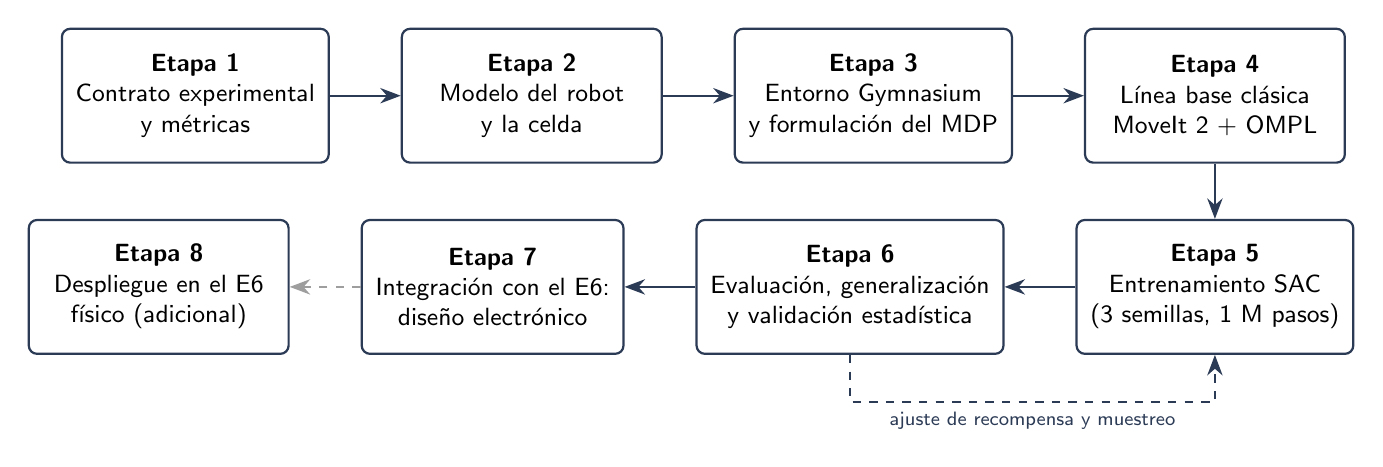
\begin{tikzpicture}[node distance=7mm and 9mm]
\ifresaltar\tikzset{b/.style={alcance,minimum width=3.3cm,minimum height=1.7cm},f/.style={fuera,minimum width=3.3cm,minimum height=1.7cm}}\else\tikzset{b/.style={bloque,minimum width=3.3cm,minimum height=1.7cm},f/.style={bloque,minimum width=3.3cm,minimum height=1.7cm}}\fi
\node[b] (e1) {\textbf{Etapa 1}\\Contrato experimental\\y métricas};
\node[b,right=of e1] (e2) {\textbf{Etapa 2}\\Modelo del robot\\y la celda};
\node[b,right=of e2] (e3) {\textbf{Etapa 3}\\Entorno Gymnasium\\y formulación del MDP};
\node[b,right=of e3] (e4) {\textbf{Etapa 4}\\Línea base clásica\\MoveIt 2 + OMPL};
\node[b,below=of e4] (e5) {\textbf{Etapa 5}\\Entrenamiento SAC\\(3 semillas, 1 M pasos)};
\node[b,left=of e5] (e6) {\textbf{Etapa 6}\\Evaluación, generalización\\y validación estadística};
\node[b,left=of e6] (e7) {\textbf{Etapa 7}\\Integración con el E6:\\diseño electrónico};
\node[f,left=of e7] (e8) {\textbf{Etapa 8}\\Despliegue en el E6\\físico (adicional)};
\draw[flecha] (e1)--(e2); \draw[flecha] (e2)--(e3); \draw[flecha] (e3)--(e4);
\draw[flecha] (e4)--(e5); \draw[flecha] (e5)--(e6); \draw[flecha] (e6)--(e7);
\draw[flechaf] (e7)--(e8);
\draw[flecha,dashed] (e6.south) -- ++(0,-6mm) -| node[pos=.25,below,etiq]{ajuste de recompensa y muestreo} (e5.south);
\ifresaltar
\node[etiq,anchor=north west] at ([yshift=-6mm]e8.south west) {\tikz{\draw[alcance] (0,0) rectangle (.5,.25);} se realiza en el curso\quad \tikz{\draw[fuera] (0,0) rectangle (.5,.25);} fuera de alcance};
\fi
\end{tikzpicture}
\end{document}
